\documentclass[]{scrartcl}

\usepackage{amsmath}
\usepackage{bbm}
\usepackage{amssymb}
\usepackage{wasysym}
\usepackage{blkarray}
\usepackage{graphicx}
\graphicspath{{images/}}
\usepackage{titlesec}
\usepackage{color}
\usepackage{tikz}
\usepackage{xfrac}
\usepackage{relsize}
\usepackage{soul}
\usetikzlibrary{calc, automata, chains, arrows.meta}
\newcommand{\1}[1]{\mathbbm{1}_{\left\{#1\right\}}}
\newcommand\independent{\protect\mathpalette{\protect\independenT}{\perp}}
\def\independenT#1#2{\mathrel{\rlap{$#1#2$}\mkern2mu{#1#2}}}
\DeclareMathOperator*{\argmax}{arg\,max}
\DeclareMathOperator*{\argmin}{arg\,min}

%\titleformat{\section}
%{\normalfont\Large\bfseries}
%{\text{Problem}\ \thesection:}{0.5em}{}


%opening
\title{High-dimensional forgeries for fun and profit}
\subtitle{A study of ``A knockoff filter for high-dimensional selective inference'' \\ Statistics 588 - Data Mining}
\author{Don Walpola}
\date{}

\begin{document}

\maketitle

In many contemporary statistical applications, variable selection is a critical component of the analysis. Variable selection is concerned with determining the optimal, in some sense, subset of available features with which to model the desired target variable. For instance, in standard linear regression, we are concerned with models of the form 
\begin{align}\label{eq:1}
	\mathbf{y} = \mathbf{\mathbf{X}}\pmb\beta + \pmb\epsilon
\end{align}
where $\mathbf{y} \in \mathbb{R}^{n}$, $\mathbf{\mathbf{X}} \in \mathbb{R}^{n \times p}$, $\pmb\beta \in \mathbb{R}^{p}$, and typically $\pmb\epsilon \sim \mathcal{N}_{n}(0, \sigma^{2} \mathbf{I}_{n})$. The columns of the design matrix $\mathbf{\mathbf{X}}$ represent the $p$ variables under consideration to model the response $\mathbf{y}$. But rather than use all $p$ features of $\mathbf{\mathbf{X}}$, we may believe that only some smaller set of $p_{0} < p$ variables are truly associated with the response $\mathbf{y}$; or in the case that $p > n$, we may seek to find the set of $p_{0} < n$ variables most strongly associated with $\mathbf{y}$ so that we can reduce our model to the identifiable case and perform regression. This is in contrast to classical statistical procedures, where inference (in the form of hypothesis testing or confidence estimates) on a pre-specified, fixed model was paramount. Issues similar to those of the classical setting must still be dealt with, however: is there a way to quantify how many of the selected variables are truly relevant features? Can we find any guarantees that the variables we select are not merely exhibiting spurious associations with the response? 
\section{Problem Description}
One way to measure the effectiveness of a variable selection procedure is by the \textit{False Discovery Rate}. Let $S = \{1, 2, \dots, p\}$ be the index set of variables under consideration, $S_{0} \subset S$ the index set of variables actually associated with the response $\mathbf{y}$, and $\widehat{S}_{0} \subset S$ the estimated index set of relevant variables produced by our variable selection procedure. The false discovery rate is defined as the expected ratio of the number of irrelevant variables we select to the overall number of variables in our estimated set:
\begin{align}\label{eq:2}
	\text{FDR} = \mathbb{E}\Bigg[\frac{\big|\{j \in S : j \in \widehat{S}_{0}\ \text{and}\ j \not\in S_{0}\} \big|}{\text{max}(|\widehat{S}_{0}|, 1)} \Bigg]
\end{align}
The quantity inside the expectation is called the \textit{false discovery proportion}, and the max function in the denominator guarantees that the ratio is defined even in the case where no variables are selected and $|\widehat{S}_{0}| = 0$. For the particular case of a linear regression model given by equation \eqref{eq:1}, the false discovery rate can be rewritten as 
\begin{align}\label{eq:3}
\text{FDR} = \mathbb{E}\Bigg[\frac{\big|\{j \in S : \widehat{\beta}_{j} \neq 0\ \text{and}\ \beta_{j} = 0\} \big|}{\text{max}(|\widehat{S}_{0}|, 1)} \Bigg]
\end{align}
Note that $\widehat{S}_{0} = \{j \in S: \widehat{\beta}_{j} \neq 0 \}$ for the linear regression model. 

\noindent
In the original formulation of the knockoff filter $\cite{ko}$, the false discovery rate is controlled by constructing a set of $p$ false, or `knockoff', variables $\widetilde{\mathbf{\mathbf{X}}}$ that replicate the covariance structure of the original variables $\mathbf{\mathbf{X}}$ both among themselves and between each knockoff $\widetilde{\mathbf{x}}_{j}$ and distinct original variable $\mathbf{x}_{k}$ for $k \neq j$, while each knockoff variable $\widetilde{\mathbf{x}}_{j}$is constructed to have correlation with its original version $\mathbf{x}_{j}$ reduced by a quantity $s_{j}$. Then a set of $p$ statistics that satisfy two properties, which will be described below, is calculated for each pair of original and knockoff variables. Finally, based on the desired false discovery rate, a cutoff threshold is computed from the data in order to select a set of variables guaranteed to not exceed the desired FDR. We now give a more detailed description following the notation used in \cite{ko, kohd}. 

\paragraph{Knockoff Procedure}
\begin{itemize}
	\item[1.] \textbf{Construct `Knockoffs'}: Let $\mathbf{\mathbf{X}} \in \mathbb{R}^{n \times p}$ be the data matrix, with the columns standardized to have unit Euclidean norm: $||\mathbf{x}_{j}||_{2}^{2} = 1$ for all columns $1 \leq j \leq p$. 
	
	The knockoff variables will be denoted $\widetilde{\mathbf{\mathbf{X}}} \in \mathbb{R}^{n \times p}$, and must satisfy the following properties:
	\begin{align*}
		\widetilde{\mathbf{\mathbf{X}}}^{T}\widetilde{\mathbf{\mathbf{X}}} = \pmb\Sigma = \mathbf{\mathbf{X}}^{T}\mathbf{\mathbf{X}}\\
		\mathbf{\mathbf{X}}^{T}\widetilde{\mathbf{\mathbf{X}}} = \pmb\Sigma - \text{diag}(\mathbf{s})\\		
	\end{align*}
	where $\text{diag}(\mathbf{s})$ is a diagonal matrix with the entries of the vector $\mathbf{s}$ along its diagonal. The vector $\mathbf{s}$ has components $s_{j}$ that quantify the reduction in correlation between an original variable and its knockoff. As described by Barber and Cand\`es $\cite{ko}$, one method for constructing such a knockoff matrix $\widetilde{\mathbf{X}}$ is to select a vector $\mathbf{s} \in \mathbb{R}^{p}_{>0}$ with all positive components such that $\text{diag}(\mathbf{s}) \preceq 2\pmb\Sigma$. Note that the partial order $\preceq$ is the \textit{Loewner order} on the convex cone of real, symmetric positive semi-definite matrices $S^{+}_{p}$:
	\begin{align*}
		&\text{For}\ \mathbf{A}, \mathbf{B} \in \mathbb{R}^{p \times p}, \quad \mathbf{A}^{T} = \mathbf{A}\ \ \text{and}\ \ \mathbf{B}^{T} = \mathbf{B}\\
		&\mathbf{A} \preceq \mathbf{B} \iff \mathbf{B} - \mathbf{A} \ \text{is positive semi-definite}
	\end{align*}
	The knockoffs are then constructed as
	\begin{align*}
		& \widetilde{\mathbf{\mathbf{X}}} = \mathbf{\mathbf{X}}(I - \Sigma^{-1}\text{diag}(\mathbf{s})) + \widetilde{\mathbf{U}}\mathbf{C}\\
		&\text{where}\quad \widetilde{\mathbf{U}} \in \mathbb{R}^{n \times p}\\ 
		&\text{such that}\ \
		\text{span}(\widetilde{\mathbf{U}}) \perp \text{span}(\mathbf{\mathbf{X}})\ \text{and}\ \  \widetilde{\mathbf{U}}^{T}\widetilde{\mathbf{U}} = \mathbf{I}\\
		&\text{and}\quad  \mathbf{C} \in \mathbb{R}^{p \times p}\\
		&\text{such that}\ \ \mathbf{C}^{T}\mathbf{C} = 2\text{diag}(\mathbf{s}) - \text{diag}(\mathbf{s})\pmb\Sigma^{-1}\text{diag}(\mathbf{s})
	\end{align*}
	The product $\mathbf{C}^{T}\mathbf{C}$ is a Cholesky decomposition, which is guaranteed to exist by the condition $\mathbf{diag}(\mathbf{s}) \preceq 2\pmb\Sigma$.
	\item[2.] \textbf{Calculate statistics $W_{j}$ for each pair of original and knockoff features $\mathbf{\mathbf{X}}_{j}$ and $\widetilde{\mathbf{\mathbf{X}}}_{j}$}:
	The statistics $W_{j}$ must satisfy the two properties of \textit{sufficiency} and \textit{anti-symmetry}.
	\begin{align*}
		&\mathit{Sufficiency}:\quad \mathbf{W} = f([\mathbf{X}, \widetilde{\mathbf{X}}]^{T}[\mathbf{X}, \widetilde{\mathbf{X}}], [\mathbf{X}, \widetilde{\mathbf{X}}]^{T}\mathbf{y})\\
		&f: S^{+}_{2p} \times \mathbb{R}^{2p} \to \mathbb{R}^{p}\\
		&\mathit{Antisymmetry}:\quad \forall S' \subset S,\\
		& W_{j}([\mathbf{X}, \widetilde{\mathbf{X}}]_{\text{swap}(S')}, \mathbf{y}) = W_{j}([\mathbf{X}, \widetilde{\mathbf{X}}], \mathbf{y})\cdot (-1)^{\1{j\in S'}}\\
		&\text{where}\ (V_{\text{swap}(S')})_{j} = \begin{cases}
		V_{j} & j \not \in S'\\
		V_{j+ p} & j \in S'
		\end{cases}
		\quad (V_{\text{swap}(S')})_{j+p} = \begin{cases}
		V_{j+ p} & j \not \in S'\\
		V_{j} & j \in S'
		\end{cases}
	\end{align*}
	Verbally, sufficiency means that the vector of statistics $\mathbf{W} \in \mathbb{R}^{p}$ depends on the concatenated data and knockoff matrix $[\mathbf{X}, \widetilde{\mathbf{X}}]$ and response vector $\mathbf{y}$ only through the covariance $[\mathbf{X}, \widetilde{\mathbf{X}}]^{T}[\mathbf{X}, \widetilde{\mathbf{X}}]$ and the marginal covariance $[\mathbf{X}, \widetilde{\mathbf{X}}]^{T}\mathbf{Y}$. Antisymmetry means that swapping the columns of a variable with its knockoff in $[\mathbf{X}, \widetilde{\mathbf{X}}]$ changes the sign of the associated statistic $W_{j}$ for that pair. 
	\item[3.]\textbf{Compute a data dependent threshold for the statistics}: For $q$ the desired FDR, $t > 0$, and $\mathcal{W} = \{|W_{j}| > 0: j \in S \}$ the set of non-zero statistics $W_{j}$, compute the threshold value:
	\begin{align*}
		T = \text{min}\Big\{t \in \mathcal{W}: \frac{1 + |j: W_{j} \leq -t|}{\text{max}(|j: W_{j} \geq t|, 1)} \leq q \Big\}
	\end{align*}
	That is, $T$ is the smallest nonzero $W_{j}$ such that the ratio of $1$ plus the number of statistics below $-T$ to the number of statistics above $T$ does not exceed the target FDR. The max function in the denominator again ensures this quantity is always defined. The other technicality of the extra $1$ added to the numerator allows some minor algebraic manipulations to make the threshold $T$ directly control the FDR - without it, a modified version of the FDR with an extra term $q^{-1}$ in the denominator is what ends up being controlled. The cost for this direct FDR control is a slightly more conservative threshold value. $T$ is then used to select a set of variables, with a guarantee that the FDR does not exceed $q$. Note that Barber and Cand\`es distinguish these two threshold values; the $T$ computed from the numerator inflated by $1$ is referred to as \textit{knockoff+}, while the $T$ derived without augmenting the numerator and which only controls the modified FDR is named the \textit{knockoff} procedure. We ignore this minor complication, and any following reference to the knockoff procedure here will be in reference to what is called \textit{knockoff+} in \cite{ko}.
\end{itemize}
There are several limitations to this procedure, some of which are addressed in $\cite{kohd}$. One limitation is that the geometrical construction of the knockoffs requires that $n \geq 2p$ (or with some augmentations, $n \geq p$). This prevents the knockoff filter from being applied to `high-dimensional' problems where $p > n$. Of course, this high-dimensional setting is arguably where variable selection is most often needed and applied. 

\noindent
A second limitation is that controlling the FDR is only practically useful in the sparse setting, where $|S_{0}| \ll |S|$. In the non-sparse setting, a more informative quantity to control would be the number of directional errors - that is, predicting $\widehat{\beta}_{j} > 0$ when in fact $\beta_{j} \leq 0$, or $\widehat{\beta}_{j} < 0$ when in fact $\beta_{j} \geq 0$. This leads to a definition of \textit{directional false discovery rate}:
\begin{align}\label{eq:4}
\text{FDR}_{\text{dir}} = \mathbb{E}\Bigg[\frac{\big|\{j \in \widehat{S}_{0} : \text{sign}(\widehat{\beta}_{j}) \neq \text{sign}(\beta_{j})\} \big|}{\text{max}(|\widehat{S}_{0}|, 1)} \Bigg]
\end{align}
Recall that the sign function takes values in the set $\{-1, 0, 1\}$, with sign$(0) = 0$. Thus, as defined, controlling the directional false discovery rate also controls the FDR because of the weak inequalities on the true parameter values $\beta_{j}$, and so FDR$_{\text{dir}}$ is also a sensible measure in sparse problems. A directional error is made when either an irrelevant variable is selected, or a relevant variable is selected but with the incorrect direction of effect. Note, however, that no distinction is made between these two types of errors by the FDR$_{\text{dir}}$.
\section{Models, Methods, Algorithms}
Barber and Cand\`es demonstrate in \cite{kohd} that, under the assumption of normally distributed observations, the knockoff filter can be used to control not just the FDR, but the FDR$_{\text{dir}}$. The subtleties and consequences of this assumption will be discussed in section 4. To explicitly address the case that $p > n$, Barber and Cand\`es $\cite{kohd}$ propose a two stage procedure:
\begin{itemize}
	\item[\textbf{1.}]\textbf{Data splitting and initial screening:} From the original, full data set $(\mathbf{\mathbf{X}}, \mathbf{y}) \in \mathbb{R}^{n \times p} \times \mathbb{R}^{n}$, select a subsample $(\mathbf{\mathbf{X}}^{(0)}, \mathbf{y}^{(0)}) \in \mathbb{R}^{n_{0} \times p} \times \mathbb{R}^{n_{0}}$ with $n_{0} < n$. The remaining data contain $n_{1} = n - n_{0}$ samples. \hl{Using some variable selection procedure, select a subset $\widehat{S}_{0} \subset S$ of features such that $|\widehat{S}_{0}| < n_{1}$.}
	\item[\textbf{2.}]\textbf{Apply Knockoff Filter on reduced model:} Using the remaining $(\mathbf{\mathbf{X}}^{(1)}, \mathbf{y}^{(1)}) \in \mathbb{R}^{n_{1} \times p} \times \mathbb{R}^{n_{1}}$ data points, reduce the model to contain only the features selected in the previous step: $(\mathbf{\mathbf{X}}_{\widehat{S}_{0}}^{(1)}, \mathbf{y}^{(1)}) \in \mathbb{R}^{n_{1} \times |\widehat{S}_{0}|} \times \mathbb{R}^{n_{1}}$, and \hl{run the knockoff procedure as previously described, but with statistics $W_{j}$ that take into account information about the signs of $\widehat{\beta}_{j}$ and $\widetilde{\beta}_{j}$.}
\end{itemize}
One thing to note is that this two stage procedure for high-dimensions must now deal with issues of conditional inference in addition to the simultaneous inference concerns of the original knockoff filter in low-dimensions. So more, and different types, of the potential pitfalls of selective inference must be dealt with $\cite{slv}$.

\noindent
In addition to issues from selective inference, the loss in statistical power associated with all data-splitting procedures is of concern. The smaller size of the subsample $(\mathbf{\mathbf{X}}^{(1)}, \mathbf{y}^{(1)})$ typically means a lowered ability to detect variables in $S_{0}$ compared to using the full dataset $(\mathbf{\mathbf{X}}, \mathbf{y})$. The naive attempt to use $(\mathbf{\mathbf{X}}_{\widehat{S}_{0}}, \mathbf{y})$ would destroy the ability of the knockoff filter to control the FDR $\cite{kohd}$. Barber and Cand\`es propose two surprising manipulations in order to regain some of the statistical power lost from data splitting:
\begin{itemize}
	\item[1.]\textit{Data Recycling}: Reuse $\mathbf{\mathbf{X}}_{\widehat{S}_{0}}^{(0)}$ when constructing the knockoff variables $\widetilde{\mathbf{\mathbf{X}}}_{\widehat{S}_{0}}$. This differs from the naive approach in that we do not construct knockoffs for $\mathbf{X}_{\widehat{S}_{0}}^{(0)}$. The knockoffs $\widetilde{\mathbf{X}}_{\widehat{S}_{0}}^{(1)}$ are constructed as usual, but we set $\widetilde{\mathbf{X}}_{\widehat{S}_{0}}^{(0)} = \mathbf{X}_{\widehat{S}_{0}}^{(0)}$, so that we have $\widetilde{\mathbf{X}}_{\widehat{S}_{0}} = \begin{bmatrix}
	\mathbf{X}_{\widehat{S}_{0}}^{(0)}\\ \widetilde{\mathbf{X}}_{\widehat{S}_{0}}^{(1)}
	\end{bmatrix}$.  
	\item[2.]\textit{Signed Statistics from Screening}: While performing the initial variable selection procedure on the data split $(\mathbf{\mathbf{X}}^{(0)}, \mathbf{y}^{(0)})$, record not just the magnitude, but also the signs of the estimated effect, $\widehat{\text{sign}}^{(0)}_{j}$, of each feature $\mathbf{\mathbf{X}}^{(0)}_{j}$ on $\mathbf{y}^{(0)}$. These initial estimates will be used to restrict the $W_{j}$ used in the knockoff filter in order to achieve the desired directional control on the reduced model.
\end{itemize}
It may seem somewhat surprising that either of these manipulations should lead to any significant increase in statistical power, but Barber and Cand\`es provide both empirical and heuristic justifications for their use. In brief, the intuition behind data recycling is the following: since the formulation of the knockoff estimate of the FDR relies on relevant features more likely to produce large $|W_{j}|$ than irrelevant features. Recycling the first $n_{0}$ data points shifts $W_{j}$ to the right, as will be described below. If the relevant features are shifted to a greater degree than null features, then we should see an increase in power - and this differential shifting is justified by distributional arguments. The justification for using the estimated signs is even more hand-wavy - as long as we believe the estimate $\widehat{\text{sign}}^{(0)}_{j}$ does in fact indicate the more likely direction of the effect of $\mathbf{\mathbf{X}}_{j}$, then the use of $\widehat{\text{sign}}^{(0)}_{j}$ for directional control has merit. Of course, this depends on the variable selection procedure used in initial screening to correctly include relevant variables and assess the direction of their effects, but typically used procedures such as the LASSO are usually believed able to do so. Care must be taken, however, as using the LASSO for initial variable screening is not guaranteed to achieve consistent recovery of the true set of relevant variables $S_{0}$ unless certain conditions restricting the covariance between relevant and irrelevant features are satisfied \cite{adlso, rndlso}. Even modifications such as the elastic net may incorrectly estimate the signs of selected features \cite{rndlso}. Such concerns are further exacerbated by the possibility that relevant features were not even in the initially considered set of $p$ features in $\mathbf{X}$, as may occur for example when causal mutations have not been typed in genome data, but mutation sites located nearby on the chromosome to, and thus correlated with, the causal mutations \textit{are} included in the observed data \cite{kohd}. Failure to recover the true support of $\pmb{\beta}$ will lead to bias in the estimates $\widehat{\pmb{\beta}}_{\widehat{S}_{0}}$, which may possibly induce directional errors. Thus the performance of the selection procedure used in the screening step is of significant concern, and will be elaborated upon in section 4.


\section{Empirical Evaluations}
The ability of the knockoff filter to control the FDR$_{\text{dir}}$ is tested on randomly generated simulated data. Barber and Cand\`es demonstrate the knockoff filter on a simulated autoregressive model and a simulated response model derived from actual genome data \cite{kohd}. In order to test the assertion (discussed in section 4 of \cite{kohd}) that FDR$_{\text{dir}}$ is controlled by the knockoff filter  for normally distributed $\mathbf{X}$ with arbitrary covariance matrix, we generate a random covariance matrix for the multivariate normally distributed $\mathbf{X}$. In order to generate an arbitrary covariance matrix that is not dominated by its diagonal entries, we use the following procedure that will generate a symmetric, positive definite matrix:
\begin{itemize}
\item[$\bullet$] First set the number of desired variables, $p$, and the number of `factors' $1 \leq k \leq p$ to generate the covariance matrix. The closer $k$ is to $p$, the closer the resulting covariance matrix will be to a diagonal matrix. Conversely, the closer $k$ is to $1$, the less like a diagonal matrix the resulting covariance matrix will be.
\item[$\bullet$] Generate a $p \times k$ matrix $\mathbf{W}$ with entries drawn from a uniform distribution. We use $\text{Uniform}[-10, 10]$ here. Also generate a $p \times p$ diagonal matrix $\mathbf{D}$ with positive diagonal entries drawn from a random distribution. We use $\text{Uniform}[1, 10]$ here.
\item[$\bullet$] Compute the covariance matrix according to the formula
$$ \mathbf{\Sigma} = \mathbf{W}\mathbf{W}' + \mathbf{D}$$
\end{itemize}
Clearly $\mathbf{\Sigma}$ is symmetric, as $\mathbf{W}\mathbf{W}'$ and $\mathbf{D}$ are symmetric. The matrix $\mathbf{W}$ can be thought of as containing $k$ `basis' vectors, as the randomly generated entries will almost certainly produce linearly independent vectors. Now this product will have at most $k$ non-zero eigenvalues, but these eigenvalues will be non-negative since standard linear algebra results shows that $\mathbf{W}'\mathbf{W}$ is positive semi-definite, and $\mathbf{W}'\mathbf{W}$ and $\mathbf{W}\mathbf{W}'$ have the same non-zero eigenvalues. Although this basis is not orthogonal like an eigenbasis, it is diagonalizable and adding the diagonal matrix will make sure that all the eigenvalues of $\mathbf{\Sigma}$ will be positive. Thus we have produced a symmetric positive-definite matrix, which we may now use as a covariance matrix. The following heat map indicates the relative magnitudes of a $500 \times 500$ matrix generated in this manner with $k = 20$ and obviously $p = 500$. 

\begin{figure}[h]
	\centering
	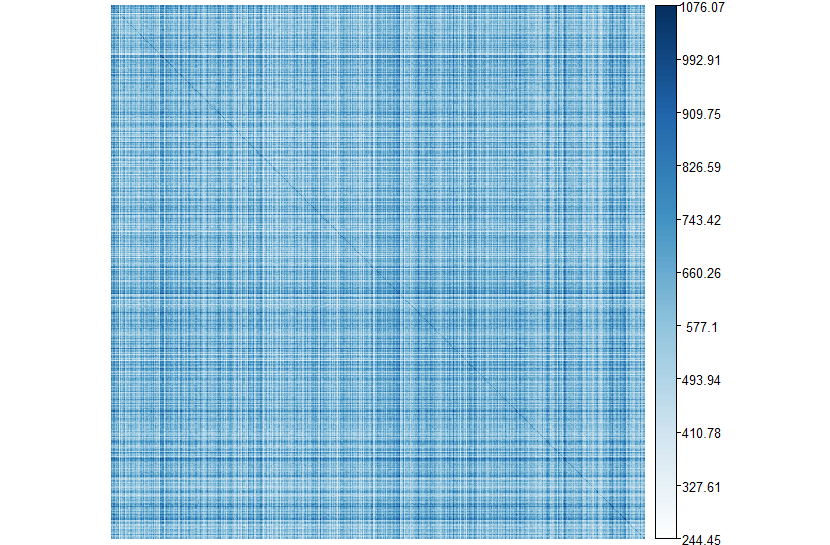
\includegraphics[width=\textwidth]{CovMat1}
	\caption{Heatmap of randomly generated $500 \times 500$ covariance matrix using $k = 20$ random `factors' with entries drawn uniformly from $[1, 10]$.}
\end{figure} 
The image was generated using the $\texttt{corrplot}$ function in the $\texttt{clusterGeneration}$ package in $\texttt{R}$. We can also gain a sense of the distribution of magnitudes by examining a histogram of the values of the matrix, displayed in Figure 2. The maximum entry in the matrix is $1164.36$ and the minimum is $244.42$.

\begin{figure}[h] ]\label{fig:hist}
	\centering
	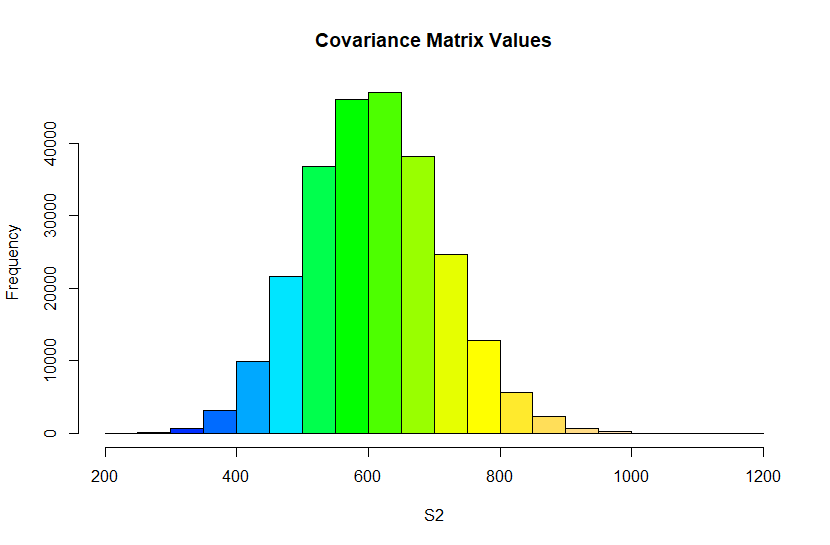
\includegraphics[width=\textwidth]{CovHist}
	\caption{Histogram of randomly generated covariance matrix entries}
\end{figure} 

A consequence of this construction is that there tends to be one principal component that accounts for the vast majority of the variance; the next $18$ to $20$ are substantially smaller, and the remaining eigenvalues of $\mathbf{\Sigma}$ are negligible in magnitude compared to the first $k$. The scree plot in figure 3 shows the variances associated with the first $50$ principal components, demonstrating this behavior. While this would be considered good behavior to have for certain forms of dimension reduction, this may lead to a high level of covariance between important and irrelevant variables. 

\begin{figure}[h]
	\centering
	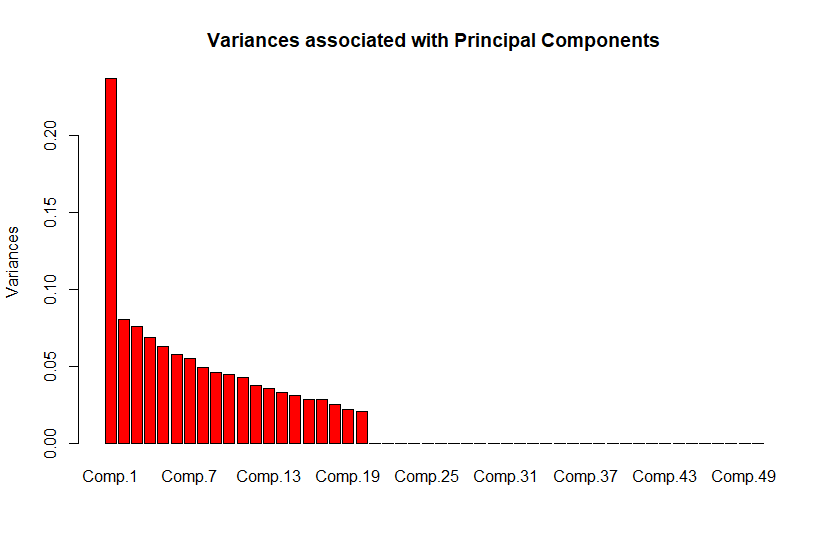
\includegraphics[width=\textwidth]{CovPCVars}
	\caption{Scree plot of variances associated with principal components of random covariance matrix generated using $p = 500$ and $k = 20$.}
\end{figure} 
Using this covariance matrix $\mathbf{\Sigma}$, we now generate the data matrix $\mathbf{X}$ using a multivariate normal distribution $\mathcal{N}(\mathbf{0}, \mathbf{\Sigma})$. As we are simulating a high-dimensional data set with fewer samples $n$ than variables $p$, we generate $n = 400$ samples and the matrix $\mathbf{X}$ is then $400 \times 500$ with each row an independent draw from $\mathcal{N}(\mathbf{0}, \mathbf{\Sigma})$. Once this is done, we normalize the data matrix so that each column has unit $L_{2}$ norm. We then randomly assign $p_{0} = 50$ of the $500$ variables to be relevant for our model, by generating a parameter vector $\pmb{\beta}$ of length $500$ and randomly selecting $50$ of its indices to be non-zero. The magnitude of the non-zero entries $\beta_{p_{0}}$ are all equal, but the signs are randomly distributed using a symmetric Bernoulli distribution. Also called a Rademacher distribution, it takes the values $-1$ and $1$ with equal probability. 

Using the generated design matrix, we now simulate a response according to the equation $y = \mathbf{X}\pmb{\beta} + \pmb{\epsilon}$, where $\pmb{\epsilon} \sim \mathcal{N}(\mathbf{0}, \sigma^{2}\mathbf{I})$. In order to assess the average performance, we apply the two-stage knockoff procedure for $100$ trials using the current magnitudes for the non-zero $\beta_{p_{0}}$. At each trial the noise vector $\pmb{\epsilon}$ is newly generated and the subsample $n_{0}$ used for initial screening is randomly drawn. The initial variable screening is performed using LASSO regression as implemented by the $\texttt{glmnet}$ function in \texttt{R}. The knockoff statistic used during the second stage is the difference in magnitudes of LASSO regression coefficients in the reduced, screened model, $|\hat{beta}_{j}| - |\tilde{\beta}_{j}|$. Several functions in the \texttt{knockoff} package were used to perform the filtering at the second stage. To assess the performance for various coefficient magnitudes, we repeat this whole procedure for a range of signal magnitudes $|\beta_{p_{0}}|$. The results are plotted against the parameter values in figure 4. We see that the directional FDR is fairly consistent, and below the set level of 0.1 used for the simulations. Directional and standard measures of power are the same, supporting the claim that the knockoff filter controls directional error rates without modification. Power was measured as the fraction of true signals finally selected after the second stage and application of the knockoff filter. Directional power further imposes that the signs of the estimate and true parameter must agree. The restricted versions considered only the true signals that made it past the initial screening stage, before the knockoff filter was applied in the second stage. The smaller denominator obviously leads to a larger magnitude for the restricted power. Weaker signal strengths are usually associated with a lower power, though it does not appear to be monotonic as a function of increasing parameter magnitude in the simulations performed. See the attached code in the file \texttt{Project Code.R} for details of the implementation.

\begin{figure}[h]
	\centering
	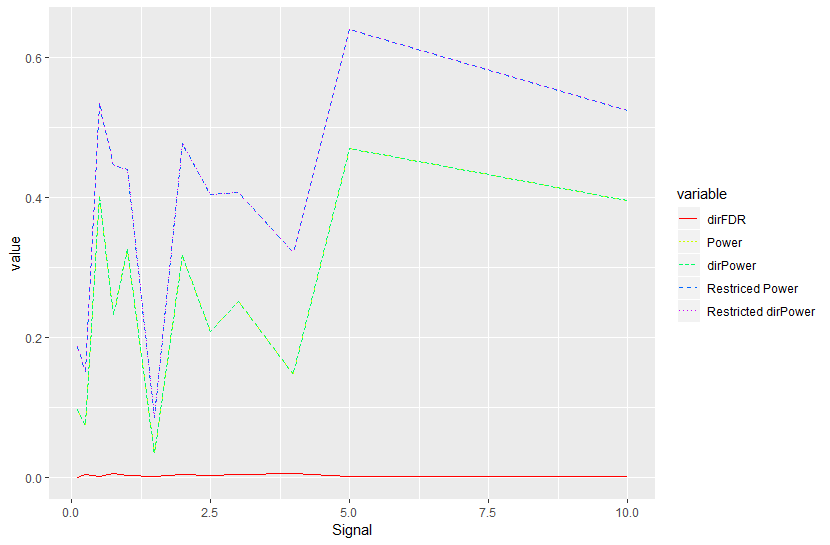
\includegraphics[width=\textwidth]{results_20}
	\caption{dirFDR and various powers as a function of true parameter magnitude.}
\end{figure}

As the average correlations between covariates are very high using the method above to generate the covariance matrix, we repeat our assessment using a slightly different covariance matrix. The only difference here is that we now take the weighted sum of two positive-semidefinite matrices as our covariance. The first matrix is generated exactly as above, while the uniform distribution used to generate the `factor' matrix $\mathbf{W}$ for the second matrix now takes values over the symmetric range $[-10, 10]$. The covariance matrix we use is then $\mathbf{\Sigma} + 2\mathbf{\Sigma}_{\text{sym}}$, with twice the weight on the matrix generated using the symmetric uniform. The resulting matrix has a lower average value for the off-diagonal terms. Unlike the earlier covariance matrix, however, some of the entries here are negative, producing a qualitatively different covariance structure. 

\begin{figure}[h]
	\centering
	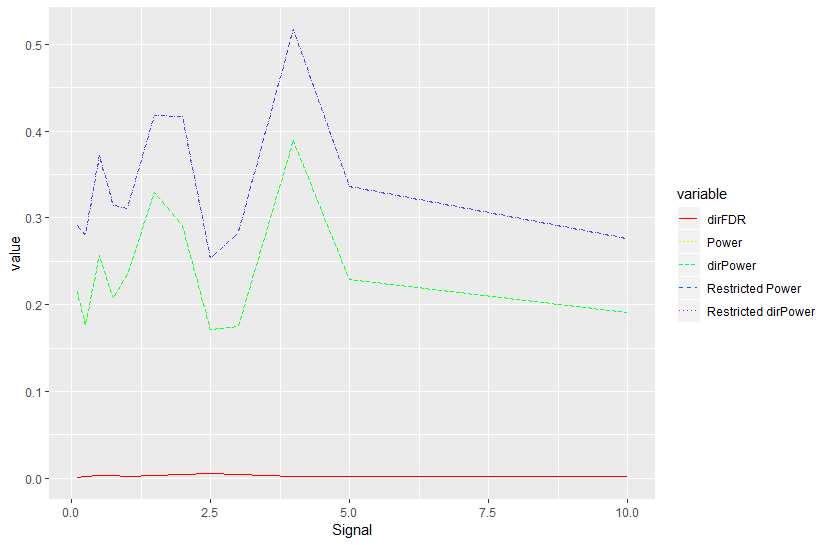
\includegraphics[width=\textwidth]{results_mixedcv}
	\caption{dirFDR and various powers as a function of true parameter magnitude, using the weighted sum covariance matrix}
\end{figure}
The results show that the dirFDR control is maintained, while all the average power measures are somewhat elevated. This should not be surprising, as the reduced amount of correlation between some of the variables will lead to better screening and selection by the LASSO. Note again, however, that the power is not monotonic with the magnitude of the true parameters. 


To test the assertion that the normality of $\mathbf{X}$ is only used  to ensure that the residuals for the partial regression performed after initial screening are still normally distributed in the proof of theorem 3 in \cite{kohd}, we use a non-normal distribution to generate the design matrix. Specifically, we use the multivariate log-normal distribution to generate $\mathbf{X}$. As this distribution is sub-exponential, the heavier tails should provide somewhat of a test to the validity of the assertion that the procedure is robuse to non-normality. The noise $\pmb{\epsilon}$ is still normally distributed to generate the response $\mathbf{y} = \mathbf{X}\pmb{\beta} + \pmb{\epsilon}$, as this is an assumption of the linear regression model. We use the \texttt{rlmvnorm} function in the \texttt{dmutate} package in \texttt{R} to draw random samples from a multivariate log-normal distribution. The covariance matrix we use for the distribution is generated in the same way as above.
\begin{figure}[h!]
	\centering
	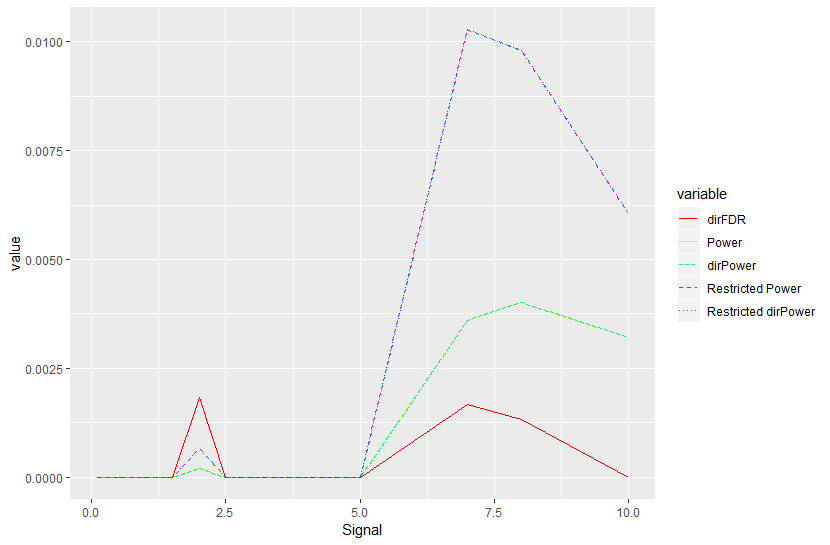
\includegraphics[width=\textwidth]{results_lgnrm1}
	\caption{dirFDR and various powers as a function of true parameter magnitude, design matrix generated using log-normal distribution}
\end{figure}
 As indicated by the plot in Figure 6, the general performance is generally poorer when compared to the previous two simulations. The scale along the y-axis shows that while the dirFDR does clearly remain below the chosen level of 0.1, all four measures of power here never exceed that level either. The compounded effects of a covariance matrix with a high average value for its off-diagonal entries and the heavier tails of a sub-exponential distribution such as the log-normal provide a formidable challenge for any variable selection procedure, and here we see the knockoff method does indeed run into difficulty. In order to see if the log-normal distribution may be responsible for more of the difficulty, we re-ran the simulation using a covariance matrix that was closer to being a diagonal matrix by using a $\mathbf{W}$ that only draws entries from the symmetric interval $[-10, 10]$ and setting the number of columns $k$ of $\mathbf{W}$ to be $1000$, so that the rank of $\mathbf{W} \mathbf{W}'$ is not deficient. 
 
 \begin{figure}[h!]
 	\centering
 	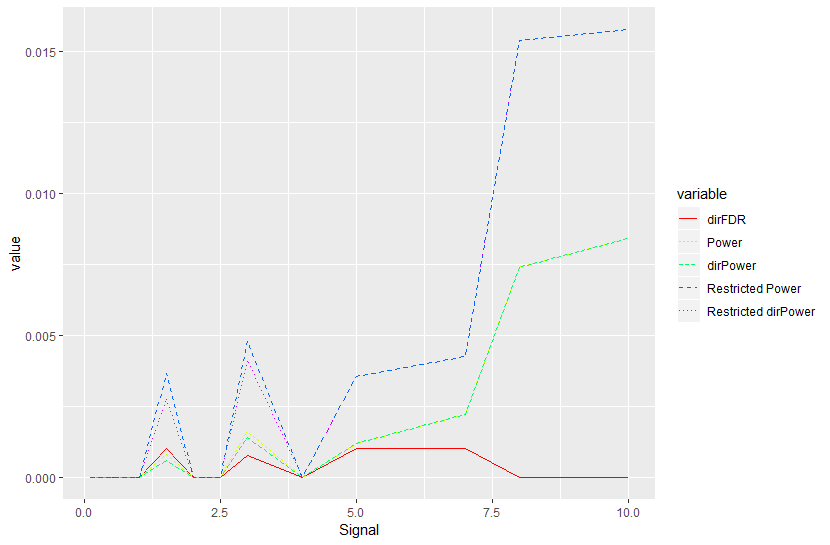
\includegraphics[width=\textwidth]{results_lgnrm2}
 	\caption{dirFDR and various powers as a function of true parameter magnitude, design matrix generated using log-normal distribution and `closer-to-diagonal' covariance matrix}
 \end{figure}
Figure 7 indicates that there is only a slight improvement in power, if any at all. Finally, we generate a design matrix from a multivariate log-normal distribution with identity covariance matrix. 
 \begin{figure}[h!]
	\centering
	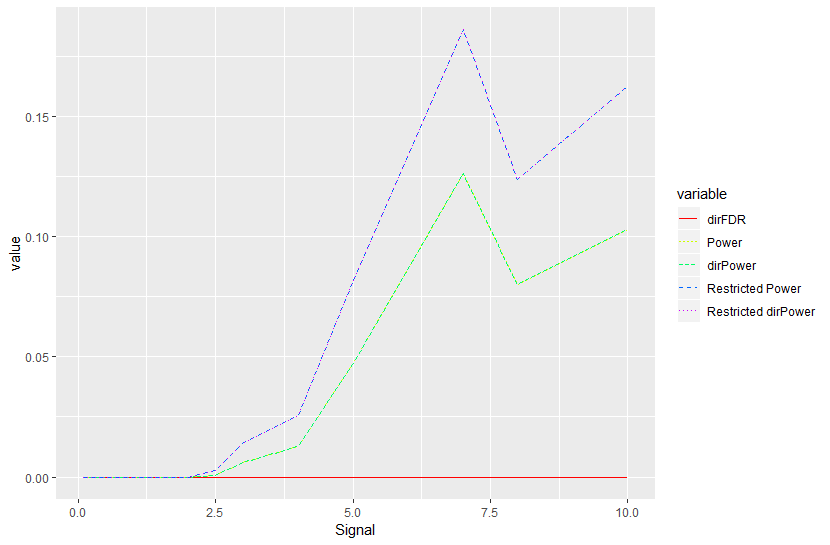
\includegraphics[width=\textwidth]{results_lgnrm3}
	\caption{dirFDR and various powers as a function of true parameter magnitude, design matrix generated using log-normal distribution and `closer-to-diagonal' covariance matrix}
\end{figure}
As Figure 8 shows, while the performance in terms of power is somewhat better here than the other two log-normal simulations, we still have substantially worse performance than when the design matrix comes from a normal distribution. This suggests that designs from a sub-exponential design, or at least a log-normal, with its heavier tails than the normal distribution, do limit the ability of the knockoff filter to make discoveries. Of course, the dirFDR is maintained below the chosen level of $0.1$ in all cases, so the knockoff filter maintains the ability to guarantee that its discoveries are not false, even if these discoveries do become much fewer under a non-normal design.
\section{Theoretical Guarantees}
The extension of the knockoff filter of \cite{ko} to the case $p > n$ in \cite{kohd} utilizes two generalizations. The first generalization is from control of FDR to control of FDR$_{\text{dir}}$. The second generalization requires guaranteeing this control is maintained even if an initial stage of model reduction is performed before applying the knockoff filter. As mentioned in section 2, in order to prove these results for directional control of the knockoff filter, assumptions of normality are made on the observations in \cite{kohd}.  These distributional assumptions on $\mathbf{y}$ or $\mathbf{X}$ are considerably stronger than the typical normality assumptions on the residuals $\pmb{\epsilon}$ used to justify the use of linear regression.  


\noindent
There are three theorems demonstrating these generalizations in \cite{kohd}. 
\begin{itemize}
	\item\textbf{Theorem 1} shows that, under the assumption that $\mathbf{y} \sim \mathcal{N}_{n}(\mathbf{X}\pmb{\beta}, \sigma^{2}\mathbf{I}_{n})$, the standard knockoff filter developed in \cite{ko} controls FDR$_{\text{dir}}$ when using $\widehat{\text{sign}}_{j} = \text{sign}\big((\mathbf{X}_{j} - \widetilde{\mathbf{X}}_{j})^{T}\mathbf{y}\big)$ as the estimated direction of effect for feature $j$. Note that this theorem applies in the same low-dimensional realm of $n \geq 2p$, and so shows that the original knockoff filter is more powerful than shown in \cite{ko}.
	\item\textbf{Theorem 2} again assumes that $\mathbf{y} \sim \mathcal{N}_{n}(\mathbf{X}\pmb{\beta}, \sigma^{2}\mathbf{I}_{n})$ and uses the same directional estimator $\widehat{\text{sign}}_{j}$ as in theorem 1. Here, however, we are in the high-dimensional setting $p > n$, and thus must use an initial screening step before applying the knockoff filter. Theorem 2 asserts that the knockoff filter controls FDR$_{\text{dir}}$ even after model reduction by some initial variable screening is performed -- conditional on a \textit{sure screening} event
	\begin{align}
		\mathcal{E} = \{\text{support}(\pmb{\beta}) \subset \widehat{S}_{0}\ \text{and}\ |\widehat{S}_{0}| \leq  \mathlarger{\sfrac{n_{1}}{2}} \}.
	\end{align}
	Note that $\1{\mathcal{E}}$ is a function of $\mathbf{y}^{(0)}$ for fixed $\mathbf{X}$, and so we are implicitly conditioning on the subsample used during preliminary screening. The result is
	\begin{align}
		\mathbb{E}[\text{FDR}_{\text{dir}}\,|\,\mathcal{E}] \leq q
	\end{align}
	\item\textbf{Theorem 3} extends these results to directional control of the linear regression parameters. Here the knockoff filter is employed with data recycling after initial screening. This, however, is demonstrated under the stronger assumption that the rows of $\mathbf{\mathbf{X}}$, denoted $\mathbf{\mathbf{X}}_{[i]}$ for $1 \leq i \leq n$, are i.i.d. samples from a multivariate Gaussian distribution,
	\begin{align}\label{eq:xn}
	\mathbf{\mathbf{X}_{[i]}} \overset{\text{iid}}{\sim} \mathcal{N}_{p}(\pmb{\nu}, \pmb{\Psi})
	\end{align}
	where $\pmb{\nu} \in \mathbb{R}^{p}$ and $\pmb{\Psi} \in \mathbb{R}^{p \times p}$ are unknown. The directional control guaranteed here is also modified to refer to the {\color{red}{\textit{partial}}} regression coefficients of the reduced set $\mathbf{\mathbf{X}}_{\widehat{S}_{0}}$ {\color{red}{\textit{expected}}} after initial screening on $(\mathbf{X}^{(0)}, \mathbf{y}^{(0)})$:
	\begin{align}
		\pmb{\beta}^{\text{\scriptsize{partial}}} = \big[\mathbf{X}_{\widehat{S}_{0}}^{(1)T}\mathbf{X}_{\widehat{S}_{0}}^{(1)} \big]^{-1}\mathbf{X}_{\widehat{S}_{0}}^{(1)T}\mathbb{E}\big[\mathbf{y}^{(1)}\,|\,\mathbf{X}_{\widehat{S}_{0}}^{(1)}; \mathbf{X}^{(0)}, \mathbf{y}^{(0)} \big]
	\end{align}
	As in theorem 2, conditioning is required on the subsample used for initial screening and the resulting model selection performed as a result. These conditioning arguments place the guarantees of the knockoff filter in high-dimensions more firmly in the field of selective inference \cite{slv}.
	
	\noindent
	Observe that in general we may have $\text{sign}(\beta_{j}) \neq \text{sign}(\beta_{j}^{\text{partial}})$. We are still tracking meaningful directional errors, however, as $\text{sign}(\beta_{j}^{\text{partial}})$ is the sign of the \textit{true partial regression} coefficient for feature $j$ if only the features in $\widehat{S}_{0}$ are used. While these may not be the same directional effects for the model using the true set $S_{0}$, using these partial regression coefficients mitigates the possibility that some relevant features were either dropped by initial screening or not even included in the observed set $S$. Thus the method still yields useful information. As mentioned by the authors, the normality assumption \eqref{eq:xn} is used so that their proof readily reduces any errors of omission in selecting $\widehat{S}_{0}$ to a type of omitted variable bias familiar from standard linear regression, and a similarly recognizable change of variance for the estimate $\pmb{\beta}^{\text{partial}}$ depending on the covariances of the selected $\widehat{S}_{0}$ and omitted $\widehat{S}_{0}^{c}$ variables. 
\end{itemize}


\noindent
Theorem 3 is the overall main result, at least from a practical perspective. As the knockoff filter is intended to find relevant features while placing a ceiling on the FDR$_{\text{dir}}$, this result most directly describes the theoretical guarantees desired to hold in practice. For this reason, the conditional nature of the statement is of major import. Both the efficacy of the selection procedure and the subsample $(\mathbf{X}^{(0)}, \mathbf{y}^{(0)})$ used for variable screening may have a potent impact on the results of the knockoff filter. Some form of cross-validation or bootstrap sampling may serve to diminish potential negative impacts incurred in this screening stage, if appropriate for the application \cite{rndlso}. This also illustrates the inapplicability of this form of the knockoff filter to problems of causal inference \cite{kohd}. The guarantees demonstrated are for $\pmb{\beta}^{\text{partial}}$ relative to $\widehat{S}_{0}$. Causal inference in this context would be concerned with guarantees regarding $S_{0}$ and $\pmb{\beta}_{S_{0}}$, which as mentioned, are deferred to the selection procedure and sample used for variable screening (and the inclusion of any causal variable in the full data matrix $\mathbf{X}$ whenever a confounder for that causal variable is included). 
\section{Discussion}
While the methods developed in \cite{kohd} to extend the knockoff filter to the case where $p > n$ do represent a significant improvement, there are still some obvious limitations present in the overall knockoff pipeline as described. Perhaps the most readily apparent is that the procedure as formulated is tailored specifically to linear regression models of the form in equation \eqref{eq:1}. A recent reformulation of the knockoff method using a distributional rather than geometric construction of the false variables addresses this issue and extends the knockoff framework to generalized linear models, with no restriction on the relative magnitudes of $p$ and $n$ \cite{komx}. Further, these `model-X knockoffs' are claimed to be robust to errors in estimating the distribution of $\mathbf{X}$ when generating $\widetilde{\mathbf{X}}$, in the sense that FDR control is reasonably maintained. If this leads to increased power while maintaining a controlled FDR when dealing with non-Gaussian data, this would substantially extend the applicability of the knockoff filter. As we saw in our simulations, a distribution with heavier tails such as a log-normal greatly limits the power of the knockoff filter to make discoveries, even if the FDR is maintained.

\noindent
Another point that may be of concern is the error measure used by the knockoff filter. Both FDR and FDR$_{\text{dir}}$ are defined as expected values of false discovery proportions. Depending on the application, this may not be the most salient performance measure. One alternative is the \textit{$k$-familywise error rate} ($k$-FWER), the probability of making at least $k$ false discoveries: 
\begin{align}\label{kfwer}
\mathbb{P}\big(|j: \widehat{\beta}_{j} \neq 0\ \text{and}\ \beta_{j} = 0|\ \geq k  \big).
\end{align}
The knockoff methodology can be extended to control this error rate, as well as other generalized type I error rates \cite{kofw}. 

\noindent
In certain contexts,  the knockoff procedure in high-dimensions controlling FDR$_{\text{dir}}$ is less conservative relative to the user-selected level $q$, and more powerful in detecting true signals when compared to earlier methods for controlling the false discovery rate. Including data recycling further reduces conservatism and increases statistical power. These properties are also somewhat more adaptive to the relative strengths of the noise in the observations and the signals from the true variables compared to other selective inference methods \cite{kohd}. Overall, when applied in the appropriate contexts, the knockoff filter can produce good results. When applied in inappropriate contexts, however, it performs poorly - like any misapplied tool.
\begin{thebibliography}{9}
	\bibitem{ko}
	Barber, Rina Foygel, and Emmanuel J. Candès. ``Controlling the false discovery rate via knockoffs." \textit{The Annals of Statistics} 43, no. 5 (2015): 2055-2085.
	
	\bibitem{kohd}
	Barber, Rina Foygel, and Emmanuel J. Cand\`es. ``A knockoff filter for high-dimensional selective inference." \textit{arXiv preprint arXiv:1602.03574v3} (2018).
	
	\bibitem{kofw}
	Janson, Lucas, and Weijie Su. ``Familywise error rate control via knockoffs." \textit{Electronic Journal of Statistics} 10, no. 1 (2016): 960-975.
	
	\bibitem{komx}
	Candes, Emmanuel, Yingying Fan, Lucas Janson, and Jinchi Lv. ``Panning for gold: ‘model‐X’ knockoffs for high dimensional controlled variable selection." \textit{Journal of the Royal Statistical Society: Series B (Statistical Methodology)} 80, no. 3 (2018): 551-577.
	
	\bibitem{slv}
	Taylor, Jonathan E. ``A Selective Survey of Selective Inference."
	\textit{Proc. Int. Cong. of Math. – 2018}.
	Rio de Janeiro, Vol. 3 (3005–3024)
	
	\bibitem{adlso}
	Zou, Hui. ``The adaptive lasso and its oracle properties." \textit{Journal of the American statistical association} 101, no. 476 (2006): 1418-1429.
	
	\bibitem{rndlso}
	Wang, Sijian, Bin Nan, Saharon Rosset, and Ji Zhu. ``Random lasso." \textit{The annals of applied statistics} 5, no. 1 (2011): 468.
\end{thebibliography}
\end{document}
